%!TEX root = ../main.tex

\chapter{Estimating the number of clusters}

In this chapter, we will focus on the open problem of estimating the number of clusters. Most of current clustering methods such that K-Means, Expectation-Maximisation with Gaussian mixture model or hierarchical clustering need a this parameter in input. Different methods are being used to perform a selection of the best model according to a criterion, unfortunately with a computational cost. In this work, we will try to tackle this challenge.

\section{Introduction and related work}
In previous models, we knew the number of components $K$ in the Gaussian mixture. In reality this parameter is unknown. 
Several methods exists to select the number of clusters

\subsection{Bayesian Information Criterion (BIC)}
A common method to select the number of clusters is to use the Bayesian Information Criterion given by:
\begin{equation}
  BIC(K) = -\log\ell_n(\hat\btheta^K)+K.\log(n)
\end{equation}
And select the model which minimizes the BIC. This can be done by running EM algorithm over a large number of models which is computationally expensive.
\subsection{Silhouette method}

\subsection{Elbow method}

\subsection{Gap Statistic}

\section{Our First method}

The idea is to add a regularization term on the estimation of the $n\times K$ matrix $\bTau$, the estimate of the number of clusters K will be the number of non-empty columns of $\bTau$.\

We consider a maximum number of clusters $M$, we note the convex set $A=\{\tau \in \RR^M : \sum_{k=1}^M\tau_k=1, \tau_k\geq 0 \quad \forall k \in [M] \}$ and the "indicator" function $\chi_A(.)$ defined by:


  \begin{equation*}
    \chi_A(x) =
    \begin{cases}
      0 & \text{if } x \in A,\\
      	\infty & \text{if } x = 0
    \end{cases}
\end{equation*}

We note $\bTau_{.,k}$ the $k^{th}$ column and $\bTau_{i,.}$ the $i^{th}$ line of $\bTau$. We will estimate $\bTau$ using the same equation \ref{cost_fun_pen}, \ref{optim-problems} with a regularization term:\\
\begin{align*}
F^{pen}(\btheta,\bTau)  =& \sum_{k=1}^K \bigg(\sum_{i=1}^{n} \Big\{\tau_{i,k}\log\varphi_{\bmu_{k},\bOmega_{k}}(\bx_i)+\tau_{i,k}
    \log(\pi_k/\tau_{i,k})\Big\}-\lambda_k||\bOmega_k||_{1,1}\bigg)\\ 
    &+ \sum_{k=1}^K ||\bTau_{.,k}||_{2} + \sum_{i=1}^{n} \chi_A(\bTau_{i,.})
\end{align*}
Removing the penalization on $\bOmega$:

\begin{align*}
F^{pen}(\btheta,\bTau)  =& \sum_{k=1}^K \bigg(\sum_{i=1}^{n} \Big\{\tau_{i,k}\log\varphi_{\bmu_{k},\bOmega_{k}}(\bx_i)+\tau_{i,k}
    \log(\pi_k/\tau_{i,k})\Big\}\\ 
    &+ \sum_{k=1}^K ||\bTau_{.,k}||_{2} + \sum_{i=1}^{n} \chi_A(\bTau_{i,.})
\end{align*}

 and the optimization problem:
\begin{equation}
\hat\bTau(\btheta)\in \arg\max_{\bTau} F^{pen}(\btheta,\bTau)
\end{equation}

Unfortunately, the regularization term prevents to derive explicit solution as in previous chapters. Furthermore, we cant separate the objective function since we optimize along columns and lines of $\bTau$. The objective function $F^{pen}(\btheta,\bTau)$ rewritten
$F^{pen}_{\btheta}(\bTau)$ can be split into two terms:

\begin{equation}
F^{pen}_{\btheta}(\bTau)={\large f}({\footnotesize
\bTau})+ {\large g}({\footnotesize
\bTau})
\end{equation}

with:

\begin{align*}
f(\bTau) =& 	\sum_{k=1}^K \bigg(\sum_{i=1}^{n} \Big\{\tau_{i,k}\log\varphi_{\bmu_{k},\bOmega_{k}}(\bx_i)+\tau_{i,k} \log(\pi_k/\tau_{i,k})\Big\} + \sum_{k=1}^K ||\bTau_{.,k}||_{2}\\
g(\bTau) =& \sum_{i=1}^{n} \chi_A(\bTau_{i,.})
\end{align*}

$f$ is convex and differentiable on its domain, $g$ is also convex but not smooth. We will tackle this problem by using a proximal method:

\begin{align*}
	\bTau^{k+1} =& {\bf{prox}}_{\lambda g}(\bTau^k - \lambda \nabla f(\bTau^k))\
			=& P_A(\bTau^k - \lambda \nabla f(\bTau^k))\\
			=&\argmin_{ \bTau : \forall K, \bTau^k \in A}\big( || \bTau - (\bTau^k - \lambda \nabla f(\bTau^k) ) ||^2_2 \big)
\end{align*}

The gradient of f on $\bTau$ is given by:

\begin{align*}
\bigg[\nabla_{\bTau}f(\bTau)\bigg]_{i,j} =& \bigg[\frac{\partial f}{\partial \bTau_{ij}}(\bTau) \bigg]_{i,j}\\
=& \log(\varphi_{\bmu_j,\bOmega_j}(x_i))+\log(\frac{\pi_j}{\tau_{i,j}})+\frac{\tau_{i,j}}{||\bTau_{.,j}||_2}-1
\end{align*}

We will use FISTA to accelerate the convergence

\begin{figure}
\begin{center}
\mybox{
\begin{minipage}{0.85\linewidth}
\begin{algorithmic}%\SetAlgoLined\tt\SetLine
\small
\STATE {\bfseries Input:} 
\STATE {\bfseries Output:} parameter estimate $\bTau$
\STATE {\tt 1: Initialize $t_1=1$ and $\bxi^0$ with}
\begin{align*}
\xi_{i,k}^{0}  &= \frac{\pi_k^{0}\varphi_{\bmu_k^{0},\bOmega_k^{0}}(\bx_i)}{\sum_{k'\in[K]}\pi^{0}_{k'}\varphi_{\bmu^{0}_{k'},\bOmega^{0}_{k'}}(\bx_i)}
\end{align*}
\STATE {\tt 2: {\bf Repeat}}
\begin{align*}
\bTau^k =&\argmin_{ \bTau : \forall K, \bTau^k \in A}\big( || \bTau - (\bxi^k - \lambda \nabla f(\bxi^k) ) ||^2_2 \big)\\
t^{k+1} =& \frac{1+\sqrt{1+4*(t^k)^2}}{2}\\
\bxi^{k+1} =& \bTau^k + \bigg( \frac{t^k-1}{t^{k+1}}\bigg) \big( \bTau^k - \bTau^{k-1} \big)
\end{align*}
\end{algorithmic}
\end{minipage}}
   \caption{ $\bTau$ estimation with FISTA}
   \label{algo:PEM}
\end{center}
\end{figure}

We use the algorithm of last chapter with the new estimation procedure of $\bTau$ 

\begin{figure}
\begin{center}
\mybox{
\begin{minipage}{0.85\linewidth}
\begin{algorithmic}%\SetAlgoLined\tt\SetLine
\small
\STATE {\bfseries Input:} data vectors $\bx_1,\ldots,\bx_n\in\RR^p$ and the number of clusters $K$
\STATE {\bfseries Output:} parameter estimate $\hat\btheta = \{\hat\bmu_k,\hat\bOmega_k,\hat\pi_k\}_{k\in[K]}$
\STATE {\tt 1: Initialize $t=0$, $\btheta=\btheta^0$.}
\STATE {\tt 2: {\bf Repeat}}
\STATE {\tt 3: \qquad Update the parameter $\bTau$ with previous algorithm}
\STATE {\tt 4: \qquad Update the parameter $\btheta$:}
\begin{align*}
\pi_k^{t+1}     &= \frac1n\sum_{i=1}^n \tau_{i,k}^t,\qquad \\
\bmu_k^{t+1}    &= \frac1{n\pi_k^{t+1}}\sum_{i=1}^n \tau_{i,k}^t\bx_i\\
\bSigma_{n,k}         &= \frac{1}{n^2\pi_k^{t+1}}\sum_{i=1}^n\tau_{i,k}^{t+1}(\bx_i-\hat\bmu_k^{t+1})(\bx_i-\hat\bmu_k^{t+1})^\top\\
\bOmega_k^{t+1} & \in \argmin_{ \bOmega\succeq 0} \Big\{ -\frac{1}{2}\log| \bOmega |+\frac{1}{2} tr(\bSigma_{N,k}\bOmega)+\frac{\lambda_k}{n\pi_k^{t+1}}||\bOmega||_{1,1}\Big\}
\end{align*}
\STATE {\tt 5: \qquad increment $t$: $t=t+1$}.
\STATE {\tt 6: {\bf Until} stopping rule.}
\STATE {\tt 7: {\bf Return} $\btheta^{t}$}.
\end{algorithmic}
\end{minipage}}
   \caption{Graphical lasso algorithm for Gaussian mixtures with cluster number discovery}
   \label{algo:PEM}
\end{center}
\end{figure}


\section{Sparse Weights Vector Estimation}

 We fit a model with an arbitrarily large number of components $K$ and penalyze the weights vector $\bpi$. The penalized negative log-likelihood is:
\begin{equation}
  \ell_n(\btheta)=
-\frac{1}{n}\sum_{i=1}^{n}\log\bigg\{{\sum_{j=1}^K\pi_k\varphi_{(\bmu_{j},\bSigma_{j})}(\bx_i)}\bigg\}+\lambda\sum_{j=1}^{K-1}\pi_j^{1/\gamma}\quad \gamma\geq1
\end{equation}
Such that:
\begin{equation}
  \sum_{j}^{K-1}\pi_j \leq 1 \quad \text{and} \quad \pi_{K}=1-\sum_{j}^{K-1}\pi_j
\end{equation}
and $\sum_{j}^{K-1}\pi_j^{1/\gamma}$ is not convex, to rectify it let note $\alpha_j = \pi^{1/\gamma}$, then:
\begin{equation}
\hat\balpha\in\argmin_{\balpha\in \RR^{K-1}}\bigg\{
-\frac{1}{n}\sum_{i=1}^{n}\log\Big\{{\sum_{j=1}^K\alpha^\gamma_j\varphi_{(\bmu_{j},\bSigma_{j})}(\bx_i)}\Big\}+\lambda\sum_{j=1}^{K-1}\alpha_j \color{black} \bigg\}\quad \gamma\geq1,  
\end{equation}
such that: $\sum_{j}^{K-1}\alpha_j^\gamma \leq 1\ \text{and}\ \alpha^\gamma_{K}=1-\sum_{j}^{K-1}\alpha_j^\gamma$. We denote $f_\btheta(\balpha)$ \color{black} this cost function.\\
If we note $A$ the $K-1$ dimensional unit sphere and {\large$\chi_A$} the indicator function of $A$ ($0$ in $A$, $\infty$ elsewhere), the minimization problem can be rewritten as
\begin{equation}
  \hat\balpha\in\argmin_{\balpha\in\RR^{K-1}}\{ f_\btheta(\balpha) + \chi_A(\balpha)  \}.
\end{equation}
To solve this minimization problem, we can use a proximal gradient method and Nesterov acceleration for the following iterative procedure:
\begin{align}
\hat\alpha^{t+1}
&={\text{prox}}_{\chi_A}( \balpha^t - h \nabla f_{\btheta}(\balpha^t)  )\\
&=\argmin_{x\in\RR^{K-1}}\big\{ \chi_A(x) + \frac{1}{2}||x-(\balpha^t - h \nabla f_{\btheta}(\balpha^t)) ||^2 \big\}\\
&=P_A( \balpha^t - h \nabla f_{\btheta}(\balpha^t) ).
\end{align}
This iteration procedure gives us the following algorithm
\begin{figure}[H]
\begin{center}
\mybox{
\begin{minipage}{0.85\linewidth}
\begin{algorithmic}%\SetAlgoLined\tt\SetLine
\small
\STATE {\bfseries Input:} $\btheta$
\STATE {\bfseries Output:} parameter estimate $\hat\bpi = \big(\balpha_1^\gamma,...,\balpha_{K-1}^\gamma,1-\sum_{j=1}^{K-1}\balpha_j^\gamma)^{t}$
\STATE {\tt 1: Initialize $t=0$, $s_0=1$ and $\bxi^0=(\bpi_1^{1/\gamma},...,\bpi_{K-1}^{1/\gamma})$\\}
\STATE {\tt 2: {\bf Repeat}}
\STATE {\tt 3: }
\begin{align}
\balpha^t =&P_A( \xi^t - h \nabla f_{\btheta}(\xi^t) )\\
s_{t+1} =& \frac{1+\sqrt{1+4*s_t^2}}{2}\\
\bxi^{t+1} =& \balpha^t + \bigg( \frac{s_t-1}{s_{t+1}}\bigg) \big( \balpha^t - \balpha^{t-1} \big)
\end{align}
\STATE {\tt 5: \qquad increment $t$: $t=t+1$}.
\STATE {\tt 6: {\bf Until} stopping rule.}
\end{algorithmic}
\end{minipage}}
   \caption{Estimation of $\alpha$ }
\end{center}
\end{figure}
and the final algorithm for estimating the gaussian mixture with a penalized weight vector is 
\begin{figure}[H]
\begin{center}
\mybox{
\begin{minipage}{0.85\linewidth}
\begin{algorithmic}%\SetAlgoLined\tt\SetLine
\small
\STATE {\bfseries Input:} data vectors $\bx_1,\ldots,\bx_n\in\RR^p$ and a large number of clusters $K$
\STATE {\bfseries Output:} parameter estimate $\hat\btheta = \{\hat\bmu_k,\hat\bSigma_k,\hat\pi_k\}_{k\in[K]}$
Initialize $t=0$, $\btheta=\btheta^0$
\STATE {\tt 1: Initialize $t=0$, $\btheta=\btheta^0$\\}
\STATE {\tt 2: {\bf Repeat}}
\STATE {\tt 3: Update the parameter $\bTau$}
\begin{align}
\tau_{i,k}^{t}  &= \frac{\pi_k^{t}\varphi_{\bmu_k^{t},\bOmega_k^{t}}(\bx_i)}{\sum_{k'\in[K]}\pi^{t}_{k'}\varphi_{\bmu^{t}_{k'},\bOmega^{t}_{k'}}(\bx_i)}.
\end{align}\\
\STATE {\tt 4: Update parameters $\bmu,\bSigma$}.
\begin{align}
\bmu_k^{t+1}    &= \frac1{n\pi_k^{t+1}}\sum_{i=1}^n \tau_{i,k}^t\bx_i,\\
\bSigma_k^{t+1} &= \frac1{n\pi_k^{t+1}}\sum_{i=1}^n \tau_{i,k}^t(\bx_i-\bmu_k^{t+1})(\bx_i-\bmu_k^{t+1})^\top.
\end{align}
\STATE {\tt 5: Update the parameter $\pi$ with previous algorithm}
\STATE {\tt 6: increment $t$: $t=t+1$}
\STATE {\tt 7: {\bf Until} stopping rule.}
\end{algorithmic}
\end{minipage}}
   \caption{Algorithm for estimating sparse weights vector on GMM}
\end{center}
\end{figure}
Ci-dessous, les résultats de l'algorithme d'estimation parcimonieuse des poids du mélange sur des données simulées. En vert notre algorithme et en rouge la méthode EM+BIC. En abscisse le nombre de vrais clusters, $K$. En ordonnée, le logarithme de l'erreur $\|\hat\bpi-\bpi^*\|_1$. Pour chaque $K$, 50 simulations ont été éffectuées. Nous représentons les premiers et troisièmes quartiles ainsi que la médiane.
\begin{figure}[H]
\center
  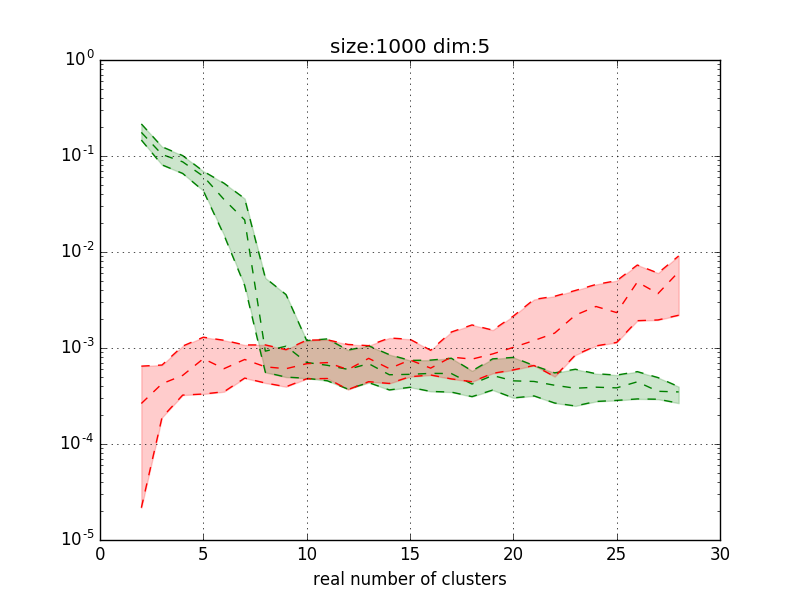
\includegraphics[width=300px]{./TeX_files/SparseWeightsVectorEstimation.png}
  \caption{Vert: Notre algorithme. Rouge: EM+BIC}
\end{figure}
